\documentclass{beamer}
\providecommand\insertframetitle{}

\usepackage{ngerman}
\usepackage{amsmath}
\usepackage{environ}
\usepackage{graphicx}
\usepackage[tikz]{bclogo}
\usepackage{tikz}
\usepackage{listings}
\usepackage{multimedia}
\usepackage{hyperref}
\usepackage{array,multirow,multicol}
\usetikzlibrary{calc}
\usepackage[utf8]{inputenc}
\usepackage[overlay,absolute]{textpos}
\usepackage{xpatch}
\usepackage{booktabs}
\usepackage{array}
\usepackage{wrapfig}
\usepackage[font=scriptsize,labelfont=bf]{caption}
\usepackage{fancyhdr}
\usepackage{enumerate}
\usepackage{enumitem}
\usepackage{gensymb}
\usepackage{setspace}

\setlist[itemize,1]{label=$\bullet$, itemsep=-1mm}
\setlist[itemize,2]{label=$\diamond$, topsep=0pt, itemsep=-1mm}



\usepackage[style=alphabetic,sortlocale=de_DE,url=false,natbib=true,backend=bibtex]{biblatex}
\beamertemplatenavigationsymbolsempty
\makeatletter
\xpatchcmd{\beamer@part}{\Hy@writebookmark{\the\c@section}{#1}{Outline\the\c@part}{1}{toc}}{}{}{}
\newcommand{\srcsize}{\@setfontsize{\srcsize}{5pt}{5pt}}
\usepackage[uni, footuni, headframelogo]{./unirostock/beamerthemeRostock}
\usepackage{graphicx}
\usepackage{multimedia}
\footinstitute{Institut für Informatik}

\addbibresource{bibliography.bib}

\title{Entwicklung von 3D-Darstellungen mit der HoloLens zur Unterstützung der Vermittlung physikalischer Inhalte}
\subtitle{Verteidigung der Masterarbeit}
\author{Matthias Kuhr}
\date{\today}

\makeatletter
\makeatother
\headLogoTop{standard} % Main-Logo (``hafen'' or ``standard'')
%\secondHeadLogoTop{20}{dbis_logo.jpg} % Optional: Image for a second logo in the header
%\showNaviSymbols % show Navi-symbols in the footer
\showNaviDots %show Navi-Dots in the header
\withParts %toogle Pagenumbering with parts on
%\printmode{handout} % Remove decoration

\begin{document}
{
	\setbeamertemplate{footline}[titlewithoutnumber] %hg%no numbers on first page
	\maketitle
	
	\nocite{Zimmer17,Milgram94}
}

%{ 
%\setbeamertemplate{footline}[titlewithoutnumber] %hg%no numbers on first page
%\begin{frame}{Gliederung}
%\begin{enumerate}
%	\item Einleitung und Zielstellung
%	\item Technischer Hintergrund
%	\item Strategien und Lösungsansätze für das Verteilungsproblem
%	\item Ergebnisse einer praktischen Umsetzung
%	\item Zusammenfassung und Ausblick
%\end{enumerate}
%\end{frame}
%}

%\part{Einleitung}
\label{part:intro}

\begin{frame}[fragile]{}
Einleitung!
\end{frame}

\part{HoloLens}
\label{part:hololens}
\begin{frame}[fragile]{}
\begin{figure}[h!]
	\centering
	\includegraphics[width=0.7\textwidth]{images/hololens.jpg}
\end{figure}
\begin{itemize}
	\pause
	\item \textit{Mixed Reality} Device
	\pause
	\item Projeziert virtuelle Objekte in das Sichtfeld des Nutzers
	\pause
	\item Nutzer bewegt sich simultan durch reale und virtuelle Szene
	\pause
	\item Genaue Bestimmung von Position und Ausrichtung im Raum durch Sensoren: \textit{Inside-Out-Tracking}
\end{itemize}	
\end{frame}

\part{State of the Art}
\label{part:sota}

\begin{frame}[fragile]{HoloLens in der Physik}
%\begin{itemize}
%	\item 
%	\item Darstellung des Wärmeprofiles bei einem erhitzten Metallstab \cite{Strzys18}	
%\end{itemize}

\begin{figure}
\includegraphics[width=0.45\textwidth]{images/Amiraslanov18.png}
\includegraphics[width=0.45\textwidth]{images/Javaheri18.png}
\begin{center}
\vspace{0.05cm}
\includegraphics[width=0.9\textwidth]{images/Strzys18.png}	
\end{center}
\setlength{\abovecaptionskip}{5pt plus 5pt minus 2pt}
\caption*{Oben Links: \citep{Amiraslanov18}, Oben Rechts: \cite{Javaheri18}, Unten: \cite{Strzys18}}
\end{figure}

\end{frame}

\begin{frame}[fragile]{Mixed Reality in der Physik}

\begin{figure}
	\includegraphics[width=0.35\textwidth]{images/Buchau09.jpg}
	\hspace{0.05cm}
	\includegraphics[width=0.35\textwidth]{images/Matsutomo13.jpg}

%	\centering
	\includegraphics[width=0.35\textwidth]{images/Buchau09_Magnet.jpg}
	\hspace{0.05cm}
	\includegraphics[width=0.35\textwidth]{images/Ibanez14.jpg}

	\setlength{\abovecaptionskip}{5pt plus 5pt minus 2pt}
	\caption*{Links: \citep{Buchau09}, Rechts Oben: \cite{Matsutomo13}, Rechts Unten: \cite{Ibanez14}}
\end{figure}

\end{frame}

\part{Problemstellung und Ziele}
\label{part:golas}

\begin{frame}[fragile]{}
Probleme und Ziele!
\end{frame}

\part{Design}
\label{part:design}

\begin{frame}[fragile]{}
Design
\end{frame}

\part{Umsetzung und Ausblick}
\label{part:practice}

\begin{frame}[fragile]{}
ASDF
\end{frame}
\part{Hintergrund und Motivation}
\label{part:intro}

\begin{frame}[fragile]{Motivation}
\vspace{10px}
\usebeamerfont{frametitle}\textcolor{blue}{Idee:} \usebeamerfont{text} HoloLens für Experimente in der Physik nutzen.
\end{frame}

\begin{frame}[fragile]{Struktur des Vortrages}
\begin{itemize}
	\item Hintergründe zur HoloLens, deren Einsatz in der Physik und zum gewählten Experiment
	\item Problemstellung
	\item Lösungsansatz
	\item Umsetzung \& Ergebnisse
	\item Diskussion
\end{itemize}
\end{frame}

\part{HoloLens}
\label{part:hololens}
\begin{frame}[fragile]{}
\vspace{-5px}
\begin{figure}[h!]
	\centering
	\includegraphics[width=0.7\textwidth]{images/papers/hololens.jpg}
\end{figure}
\pause
\begin{itemize}
	\item Projeziert virtuelle Objekte in das Sichtfeld des Nutzers
	\item Nutzer bewegt sich simultan durch reale und virtuelle Szene
	\pause
	\item Genaue Bestimmung von Position und Ausrichtung im Raum durch Sensoren: \textit{Inside-Out-Tracking}
	\item Interaktion über Gesten und Sprache, Toolkit mit vorgefertigten Objekten und Funktionen
	\pause
	\item Ermöglicht \textit{Augmented Reality} Anwendungen
\end{itemize}	
\end{frame}

\begin{frame}[fragile]{Technische Aspekte}
		\begin{itemize}
			\pause
			\item \textit{See-Through Display}, Zwei 16:9 HD Bilder, 32\degree FoV (diagonal)
			\begin{itemize}[topsep=-5px]
				\setlength{\itemsep}{-5px}
				\item Einfluss auf Größe und Farbe von Objekten
			\end{itemize}
			\pause
			\item Akkomodation der Augen fest bei 2 m
			\begin{itemize}[topsep=-5px]
				\setlength{\itemsep}{-5px}
				\item Einfluss auf Distanz
			\end{itemize}
			\pause
			\item \textit{Inside-Out Tracking} über Tiefenkamera, Stereo-Kameras und IMU
			\begin{itemize}[topsep=-5px]
				\setlength{\itemsep}{-5px}
				\item Einfluss auf Positionierung und Stabilität
			\end{itemize}
			\pause
			\item Stand-Alone Device, 1 GHz CPU/HPU, 2 GB RAM
			\begin{itemize}[topsep=-5px]
				\setlength{\itemsep}{-5px}
				\item Einfluss auf Performance
			\end{itemize}
		\pause
			\item Optimiert Stabilität der Objekte für ausgewählte Ebene
			\begin{itemize}[topsep=-5px]
				\setlength{\itemsep}{-5px}
				\item Einfluss auf Positionierung und Stabilität
			\end{itemize}
		\end{itemize}
\end{frame}

\part{State of the Art}
\label{part:sota}
\begin{frame}[fragile]{HoloLens in der Physik}
\vspace{0.1cm}
\pause
\begin{figure}
	\includegraphics[width=0.42\textwidth]{images/papers/Amiraslanov18.png}
	\includegraphics[width=0.42\textwidth]{images/papers/Javaheri18.png}
	\begin{center}
	\vspace{0.03cm}
	\includegraphics[width=0.85\textwidth]{images/papers/Strzys18.png}	
	\end{center}
	\setlength{\abovecaptionskip}{7pt plus 5pt minus 2pt}
	\caption*{Oben Links: Amiraslanov (2018), Oben Rechts: Javaheri (2018), Unten: Strzys (2018)}
\end{figure}
\end{frame}

\begin{frame}[fragile]{Augmented Reality in der Physik}
\pause
	\vspace{0.1cm}
\begin{figure}
	\includegraphics[width=0.32\textwidth]{images/papers/Buchau09.jpg}
	\hspace{0.05cm}
	\includegraphics[width=0.32\textwidth]{images/papers/Matsutomo13.jpg}

%	\centering
	\includegraphics[width=0.32\textwidth]{images/papers/Buchau09_Magnet.jpg}
	\hspace{0.05cm}
	\includegraphics[width=0.32\textwidth]{images/papers/Ibanez14.jpg}

	\setlength{\abovecaptionskip}{7pt plus 5pt minus 2pt}
	\caption*{Links: Buchau (2009), Rechts Oben: Matsutomo (2013), Rechts Unten: Ibanez (2014)}
\end{figure}
\end{frame}

\part{Anwendungsfall: Helmholtz-Spulen}
\label{part:physics}
\begin{frame}[fragile]{Experiment: Bestimmung des Erdmagnetfeldes}
\begin{minipage}{0.45\textwidth}
	\centering
	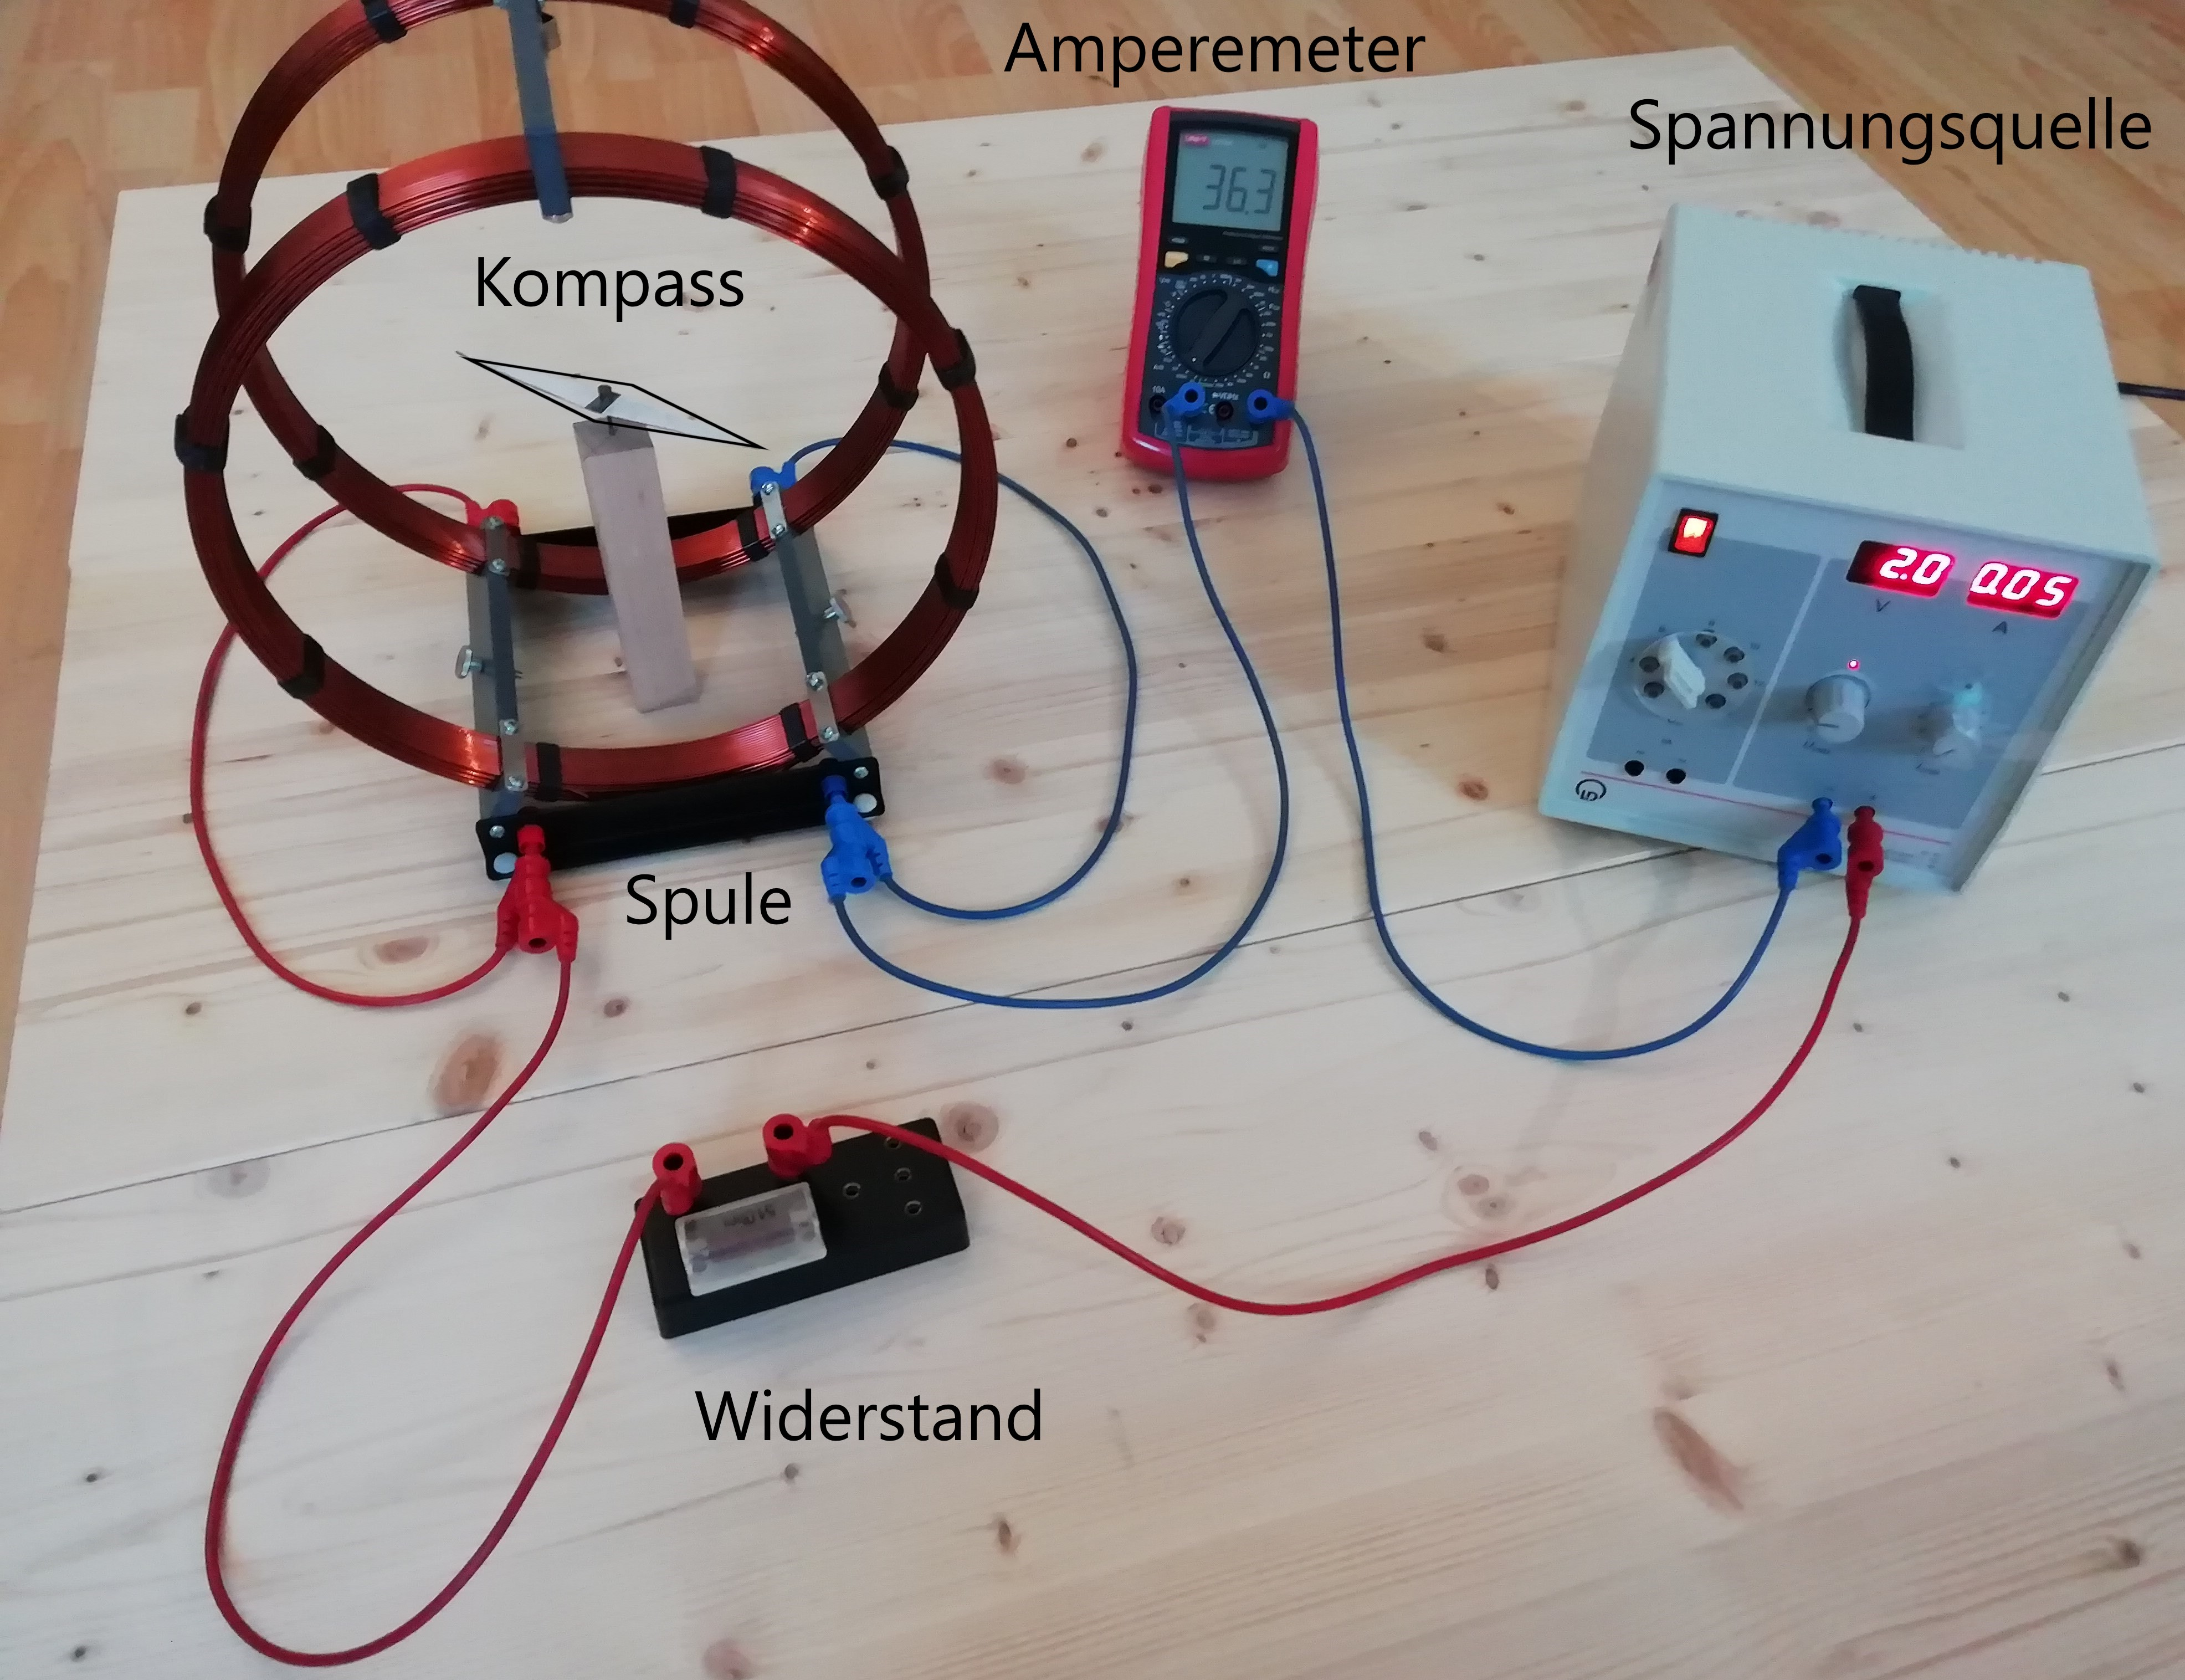
\includegraphics[width=0.9\textwidth]{images/papers/setup_labled.jpg}\\
	\small Foto des Versuchsaufbaus mit Bezeichnung der Elemente.
\end{minipage}
\pause
\begin{minipage}{0.5\textwidth}
	{\setstretch{1.0}
		\begin{itemize}[itemsep=1mm]
			\item[$1.$] Kompass ausrichten lassen
			\item[$2.$] Spule orthogonal zur Nord-Süd-Achse aufstellen
			\item[$3.$] Spannungsquelle einschalten und Stromfluss erhöhen, bis Kompassnadel um 45\degree ausgelenkt ist
			\item[$4.$] Flussdichte mit Formel aus Stromstärke und Spuleneigenschaften berechnen
		\end{itemize}
	}
\end{minipage}
\end{frame}

\begin{frame}[fragile]{Physikalischer Hintergrund}
\begin{minipage}{0.5\textwidth}
	{\setstretch{1.0}
		\begin{itemize}[itemsep=1mm]
			\item Magnetfeld ist 3D-Vektorfeld, Flussdichte $\vec{B}$ in Tesla
			\item Stromfluss durch Spule erzeugt ein Magnetfeld, abhängig von Stromstärke
			\item Helmholtz-Spule: Feld im Inneren weitgehend \textit{homogen}
			\item Feldlinien und Vektormodell sind etablierte Darstellungsmodelle
		\end{itemize}
	}
\end{minipage}
\pause
\begin{minipage}{0.45\textwidth}
	\centering
	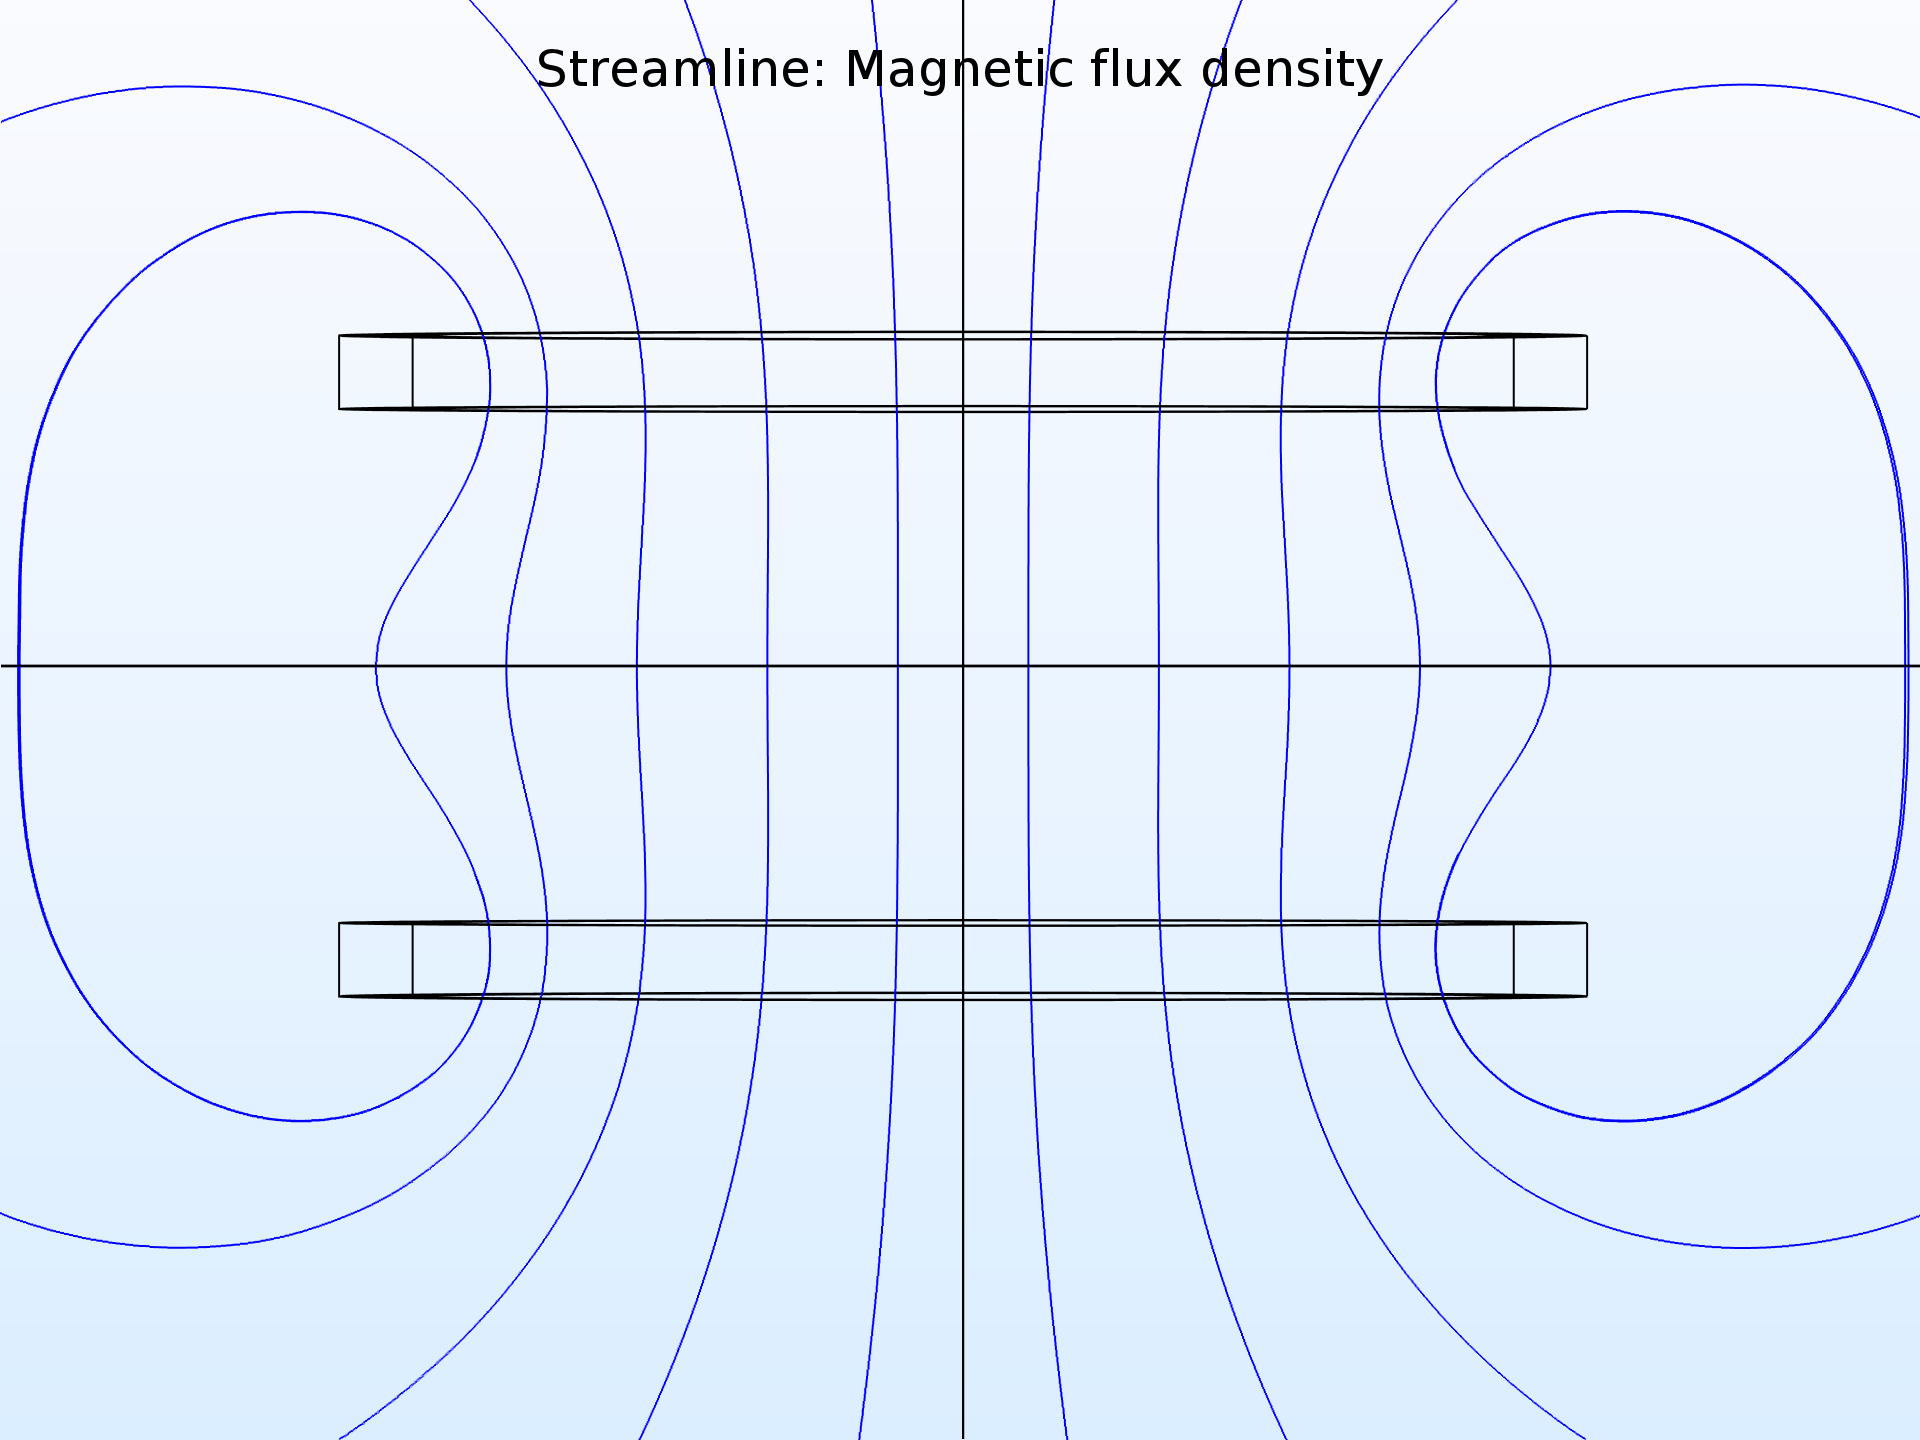
\includegraphics[width=0.9\textwidth]{images/papers/hh_mfield_nocol.png}\\
	\small Darstellung des Magnetfeldes einer Helmholtz-Spule mittels Feldlinien für eine Ebene.
\end{minipage}
\end{frame}

\part{Ziel \& Frage}
\label{part:goal}
\begin{frame}[fragile]{}
\usebeamerfont{frametitle}\textcolor{blue}{Ziel:} \usebeamerfont{text}HoloLens einsetzen, um Versuchsaufbau mit Informationen anzureichern.
\pause
\vskip 1em
\usebeamerfont{frametitle}\textcolor{blue}{Frage:} \usebeamerfont{text}Wie kann die HoloLens für diesen Versuch konkret eingesetzt werden?
\end{frame}

\part{Anforderungen}
\begin{frame}[fragile]{}
\begin{center}

\includegraphics[width=0.9\textwidth]{images/ToDo.jpg}
\end{center}
\end{frame}

\part{Physikalische Seite}
\begin{frame}[fragile]{Anforderungen aus dem Anwendungsfall heraus}
\begin{itemize}
\item Magnetfeld von Erde und Spule
\begin{itemize}
\item Stärke
\item Richtung
\item Homogenität
\item Inhomogenität am Rand der Spule andeuten (Optional) 
\end{itemize}
\item Stromfluss durch die Spule
\begin{itemize}
\item Richtung
\item Kennzeichnung von Plus und Minus
\item Stärke (Optional) 
\end{itemize}
\end{itemize}
\end{frame}

\begin{frame}[fragile]{Anforderungen aus dem Anwendungsbereich}
\begin{itemize}
\setlength{\itemsep}{-0.25em}
\item Kompass
\begin{itemize}
\setlength{\itemsep}{-0.25em}
\item Nordrichtung
\item Grobe Auslenkung der Nadel
\end{itemize}
\item Weitere Informationen (Optional)
\begin{itemize}
\item Windungszahl der Spule
\item Durchmesser und Abstand der Spulen
\item Numerische Werte und Informationen (z.B. Fließt aktuell Strom, angelegte Stromstärke, angenommene Stärke des Erdmagnetfeldes, systematischer und zufälliger Fehler, etc.)
\end{itemize}
\end{itemize}
\end{frame}

\part{Technische Seite}
\label{part:tech}
\begin{frame}[fragile]{Möglichkeiten der HoloLens}
\begin{minipage}{0.5\textwidth}
	{\setstretch{1.0}
		\begin{itemize}[itemsep=1mm]
			\item Holografische Darstellungen
			\item Raumverständnis
			\item Raumklang
			\item Interaktion
			\item Softwareunterstützung
		\end{itemize}
	}
\end{minipage}
\begin{minipage}{0.48\textwidth}
%	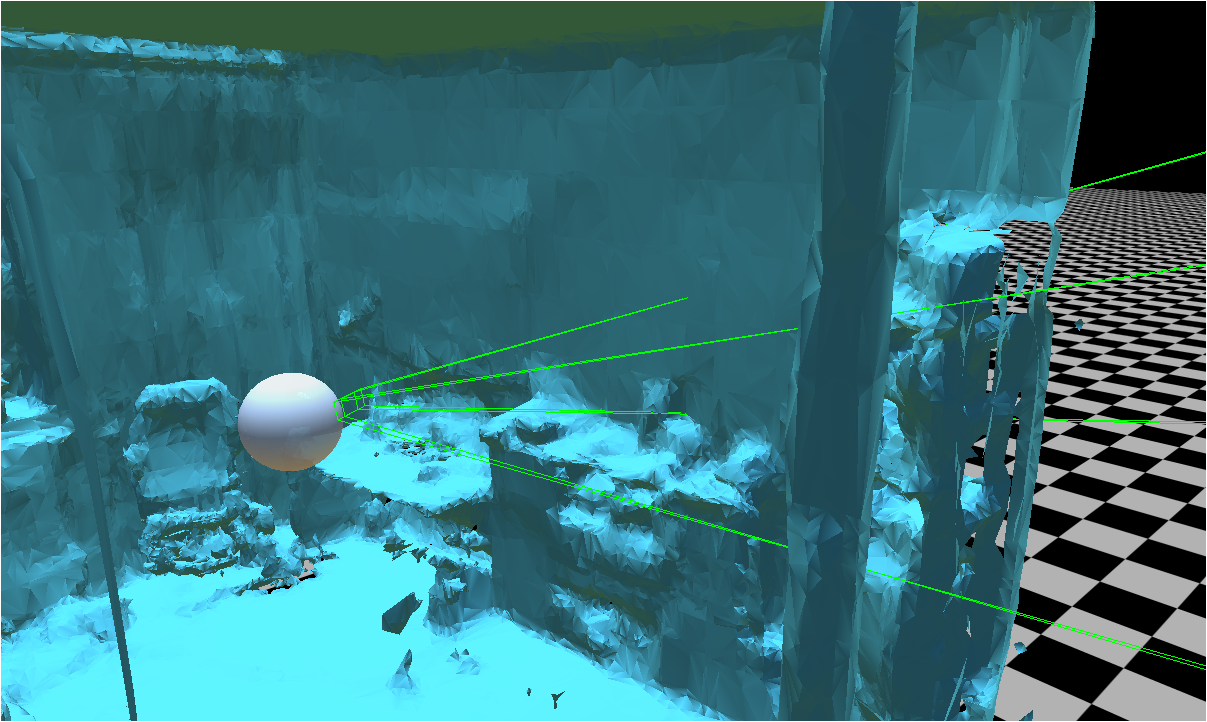
\includegraphics[width=0.9\textwidth]{images/Spatial_Understanding.png}
%	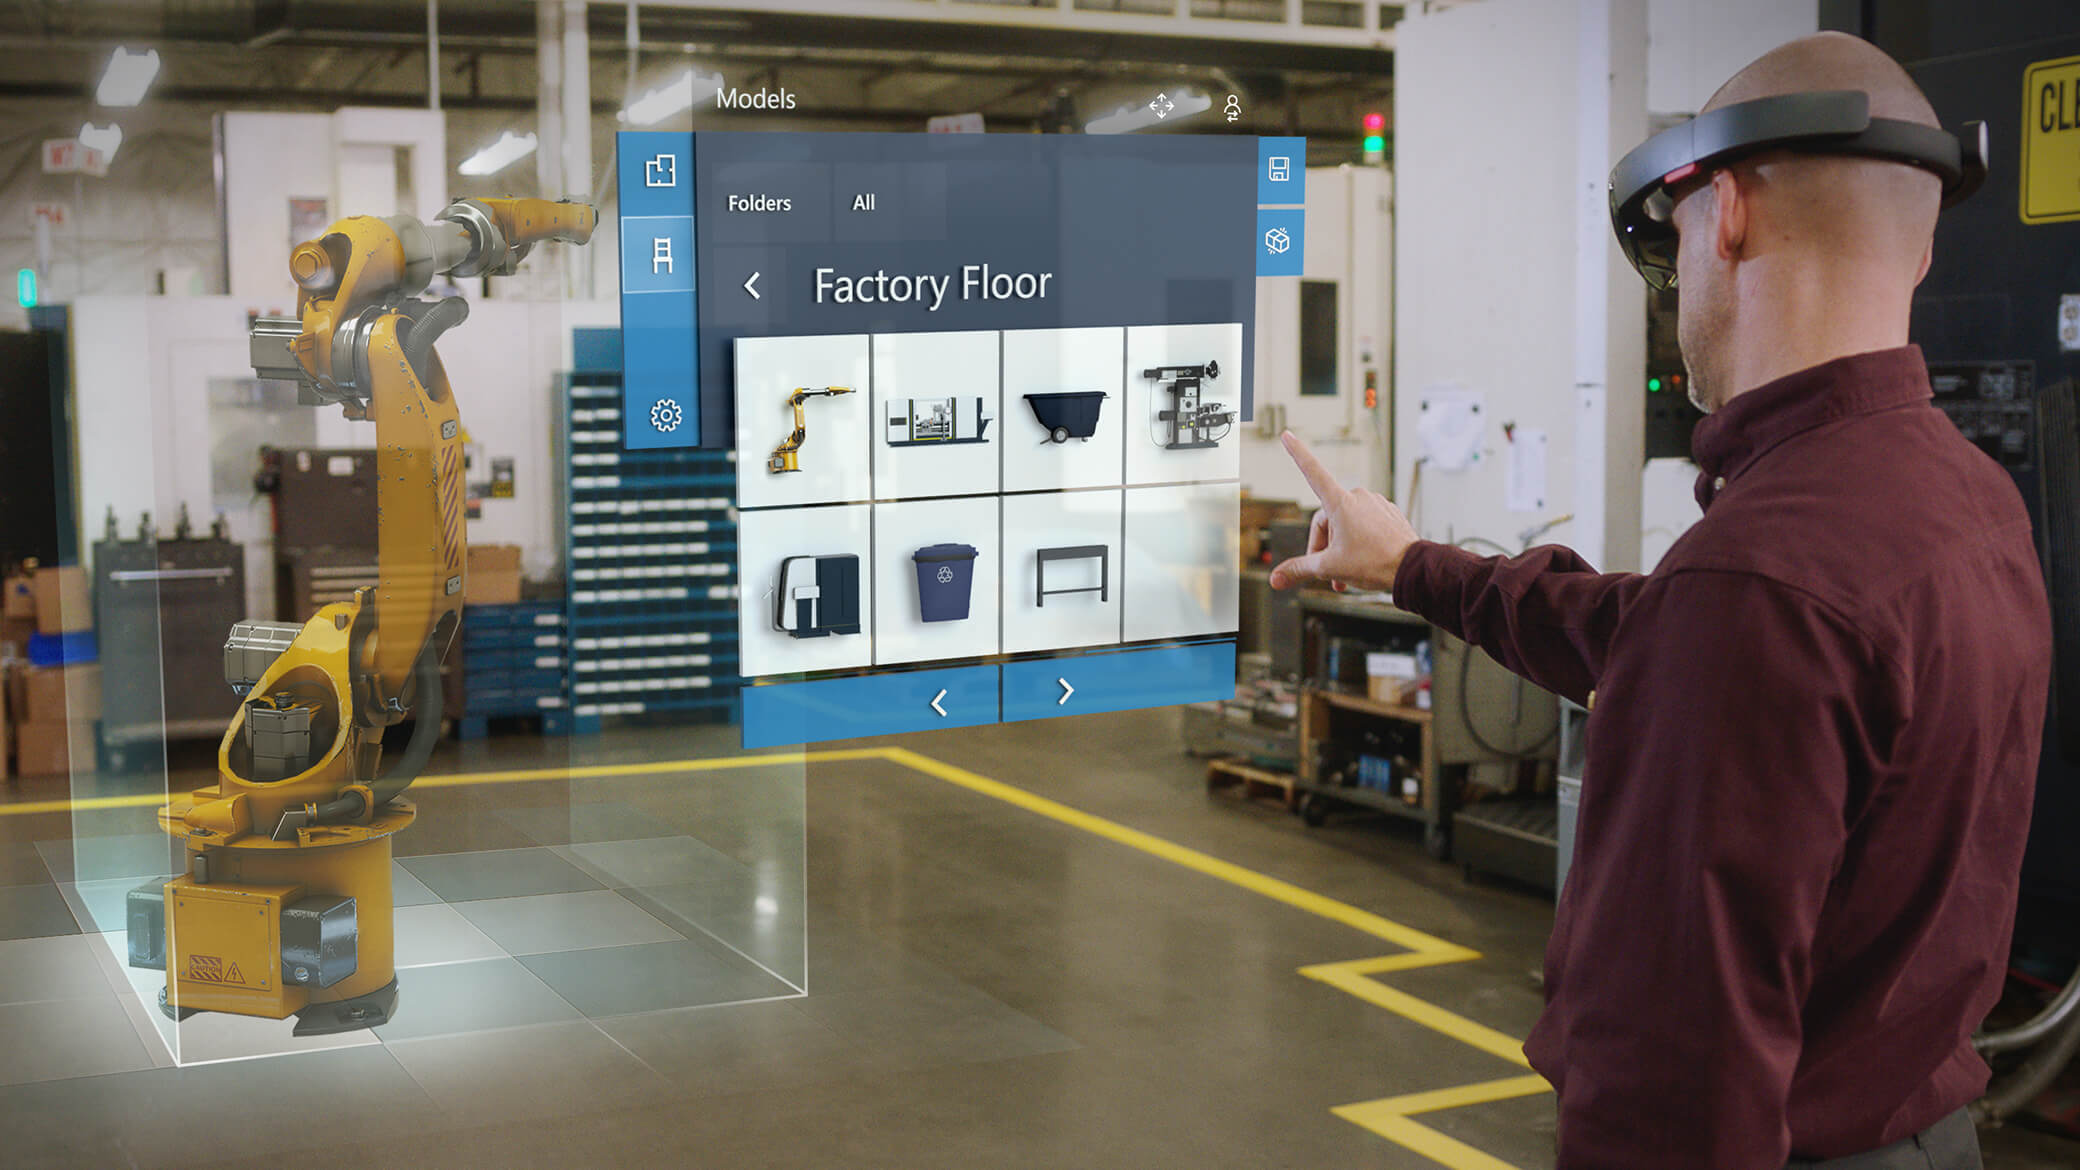
\includegraphics[width=0.9\textwidth]{images/HoloLens_Factory_Floor.jpg}
\end{minipage}
\end{frame}

\begin{frame}[fragile]{Anforderungen aus technischen Gegebenheiten}
\begin{itemize}
\item Größe, Geschwindigkeit, Farbe, Distanz zur Kamera von Objekten
\pause
\item Zusammenspiel der Darstellungen mit der Umgebung beachten
\pause
\item Stabilität der Hologramme gewährleisten
\pause
\item 60 FPS stabil halten, stark spiegelnde oder transparente Oberflächen vermeiden, mögliche Einflüsse auf die Sensoren beachten
\pause
\item Usability und UX Empfehlungen beachten
\end{itemize}
\end{frame}


\part{Problemstellung}
\label{part:golas}
\begin{frame}
\vspace{-1em}
\begin{center}
%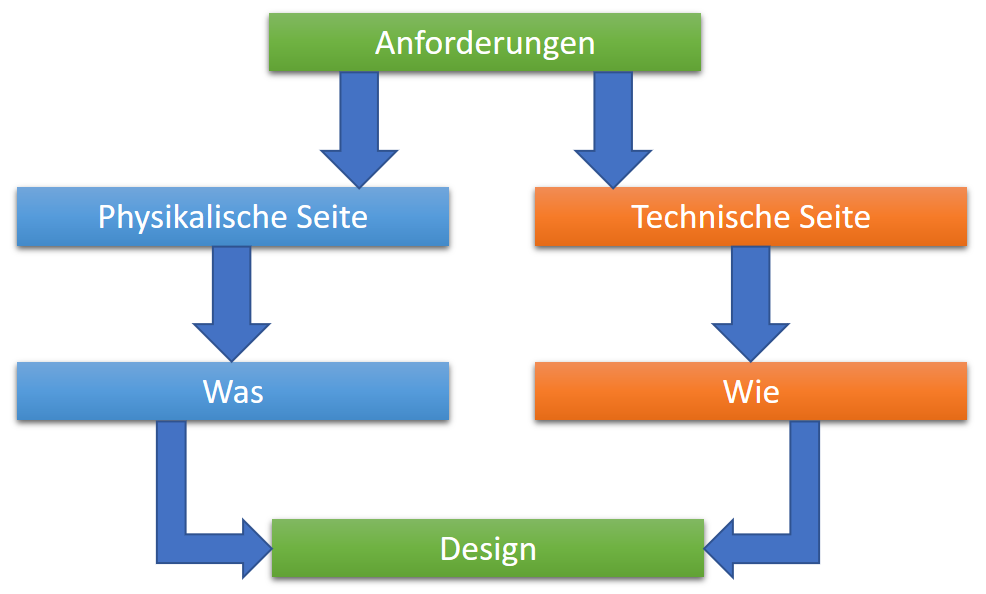
\includegraphics[width=0.8\textwidth]{images/Informiertes_Design.png}	
\end{center}
\usebeamerfont{frametitle}\textcolor{blue}{Fragen:}
\begin{itemize}
\item Was soll dargestellt werden?
\item Wie soll es dargestellt werden?
\item Wie soll damit interagiert werden?
\end{itemize}
\vspace{50px}
\end{frame}

\part{Lösungsansatz}
\label{part:solution}
\begin{frame}[fragile]{}
	\textit{Erweiternde Darstellungen erstellen und räumlich wie zeitlich in den Versuch integrieren}
	\pause
	\begin{itemize}
		\item Magnetfelder, deren Eigenschaften, Stromfluss und Auswirkung auf die Nadel anzeigen
		\item Positionierung und Stabilisierung der HoloLens nutzen		
		\item Echtzeitdaten (Messwerte) an die HoloLens übermitteln und darstellen
		\item Technische Einschränkungen beim Design berücksichtigen
	%	\begin{itemize}[topsep=-5px]
	%		\setlength{\itemsep}{-5px}
	%		\item Maßnahmen zur Vermeidung von Problemen anwenden
	%		\item Angepasstes Design
	%		\item Vorgefertigte Objekte nutzen
	%	\end{itemize}
		\item Anpassung von realen Objekten, um Integration mit der Anwendung zu verbessern
	\end{itemize}
\end{frame}

\part{Lösung}
\begin{frame}[fragile]{}
	\vspace{-10px}
	\centering
	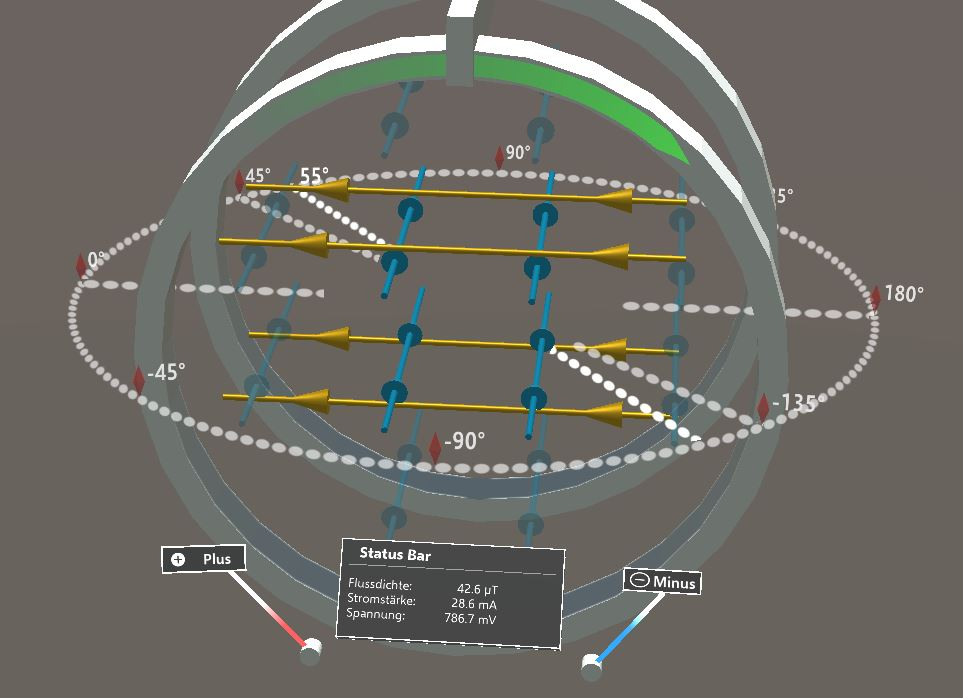
\includegraphics[width=0.75\textwidth]{images/unity/overview.jpg}\\
	\scriptsize Darstellungen in der Entwicklungsumgebung (Unity). Auflösung und Qualitätseinstellungen entsprechen den Werten auf der HoloLens.
\end{frame}

\begin{frame}[fragile]{}
\begin{figure}
	\vspace{-10px}
	\centering
	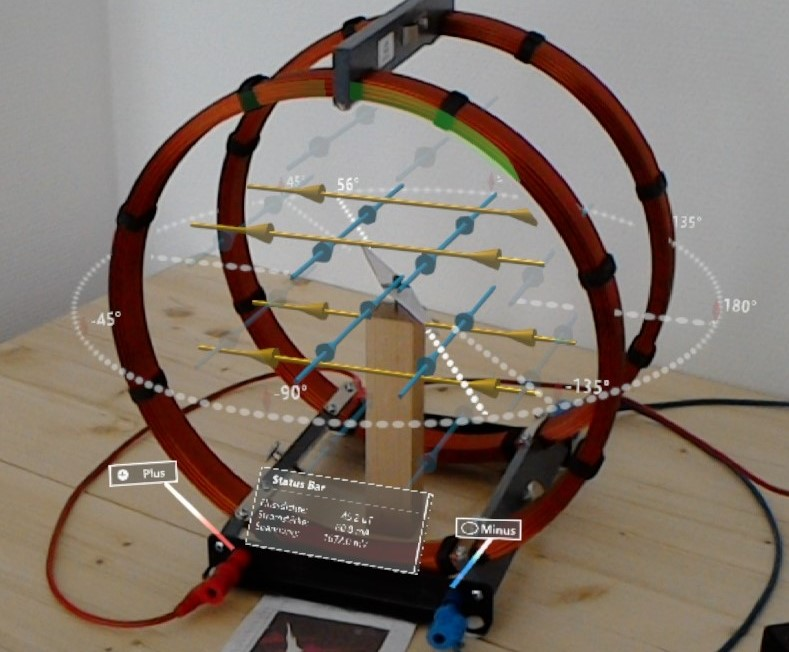
\includegraphics[width=0.7\textwidth]{images/HL/fieldlines_cut.jpg}\\
	\scriptsize Screenshot von der HoloLens mit Feldliniendarstellung.
\end{figure}
\end{frame}

\begin{frame}[fragile]{}
\begin{figure}
	\vspace{-10px}
	\centering
	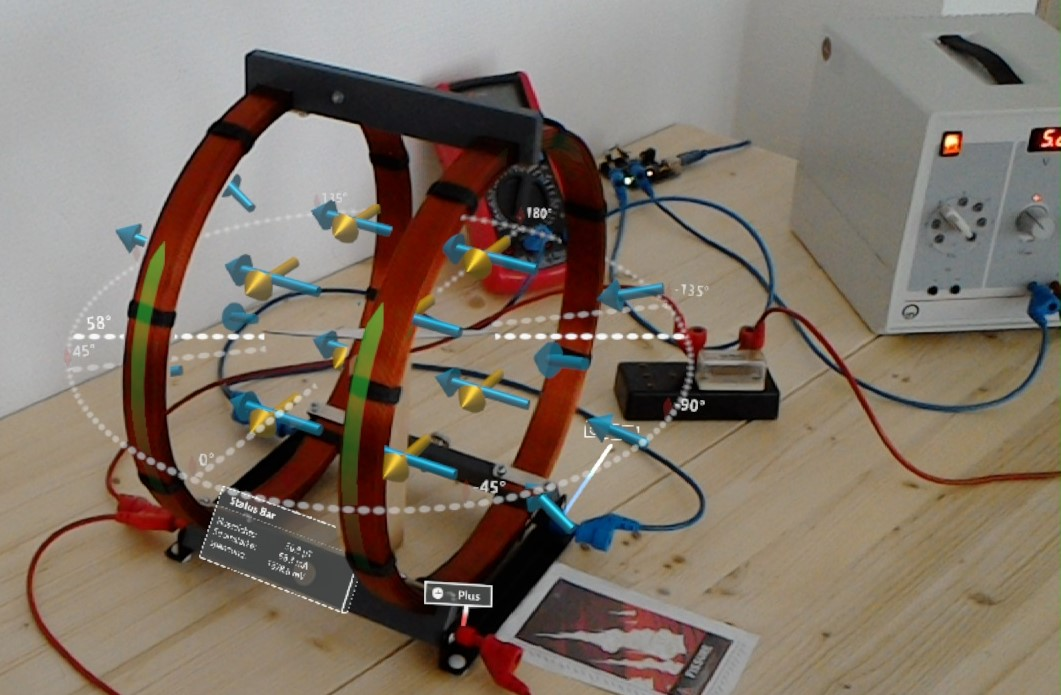
\includegraphics[width=0.85\textwidth]{images/HL/Vektoren.jpg}\\
	\scriptsize Screenshot von der HoloLens mit Vektordarstellung.
\end{figure}
\end{frame}

\begin{frame}[fragile]{Near Plane Fading}
\begin{figure}
	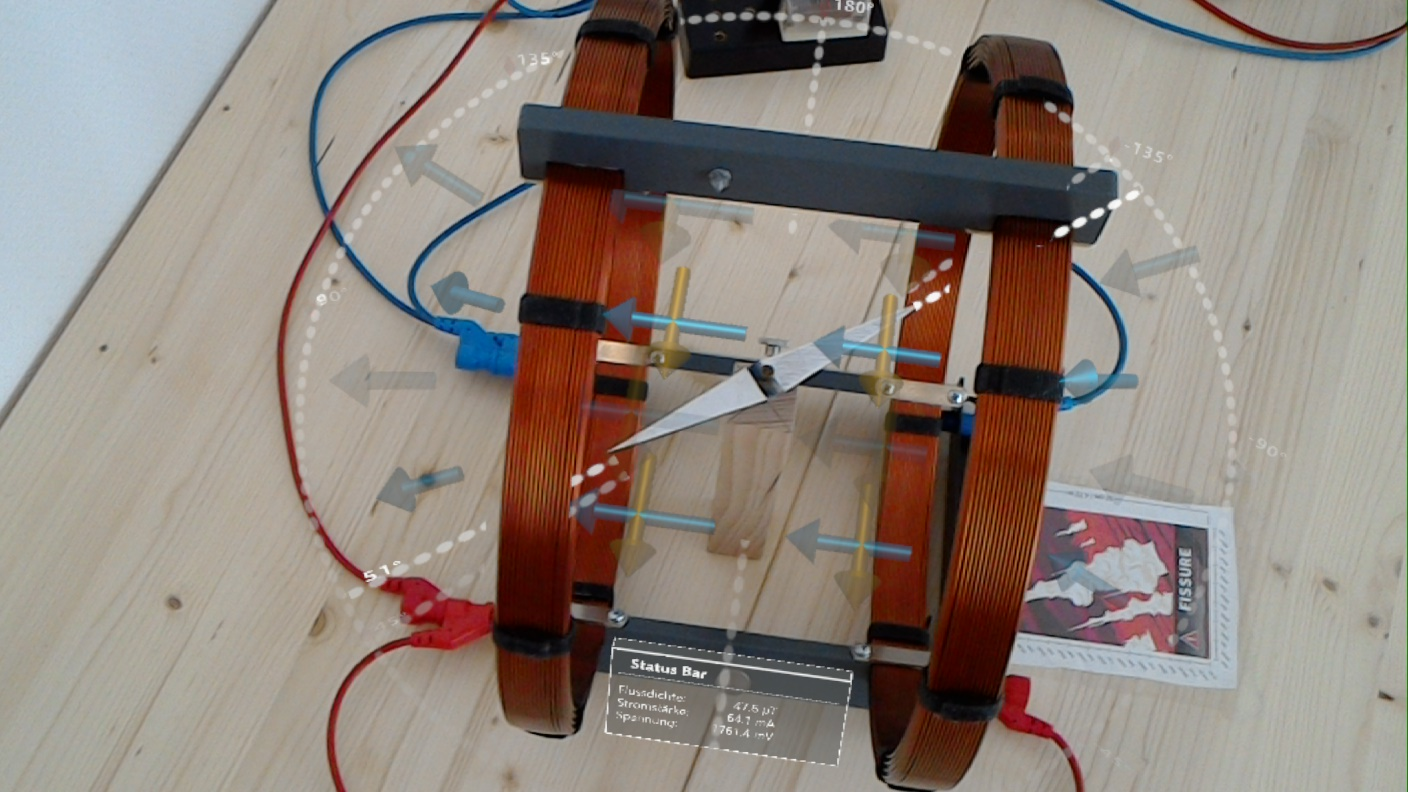
\includegraphics[width=0.8\textwidth]{images/HL/compass.jpg}
\end{figure}
\end{frame}

\begin{frame}[fragile]{Design}
\begin{itemize}
	\item Nutzung etablierter Darstellungsmodelle
	\pause
	\item Anwendung für Nutzung im Abstand von ca. 1,3 m designet, zu nah liegende Objekte werden ausgeblendet
	\begin{itemize}
		\item Hologramme passen ins Sichtfeld, sind nicht zu dicht positioniert, nutzen Screenspace aus, Komfortable Nutzung möglich
	\end{itemize}
	\pause
	\item 
	\pause
	\item Umsetzung empfohlener Maßnahmen zur Verbesserung der Performance
\end{itemize}
\end{frame}


\part{Ergebnisse}
\label{part:results}
\begin{frame}[fragile]{Erweiterungen}
\begin{itemize}
	\item Visualisierung der Komponenten des Magnetfeldes in zwei Darstellungen und in Echtzeit
	\item Darstellung einer vorberechneten Lösung für eine ausgewählte Ebene des Feldes der Spule
	\item Kennzeichnung der Stromrichtung
	\item Integration einer virtuellen Kompass-Skala mit Hervorhebung wichtiger Zustände
	\item Einbettung einer virtuellen Kompassnadel auf Basis theoretischer Werte
	\item Numerische Darstellung gemessener und berechneter Echtzeitdaten
\end{itemize}
\end{frame}


\part{Ausblick}
\label{part:future}
\begin{frame}[fragile]{Erweiterungen}
\usebeamerfont{frametitle}\textcolor{blue}{Inhaltlich:} \usebeamerfont{text}\textit{Weitere Lerninhalte integrieren}
\begin{itemize}
	\item Weitere Inhalte, z.B. Rechte-Hand-Regel
	\item Weitere Experimente, z.B. Ablenkung eines Elektronenstrahles
\end{itemize}
\pause
\vskip 1em
\usebeamerfont{frametitle}\textcolor{blue}{Technische:} \usebeamerfont{text}\textit{Portierung für HoloLens 2}
\begin{itemize}
	\item Auflösung x4 pro Auge, Sichtfeld x2 (Fläche)
	\item Tragekomfort und Interaktion verbessert
\end{itemize}

\vspace{50px}
\end{frame}



\part{Diskussion}
\begin{frame}[fragile]{}
Vielen Dank für Ihre Aufmerksamkeit!

\vspace{1em}
\hspace{1em} Fragen?
\end{frame}

\part{Umsetzung}
\begin{frame}[fragile]{Technische Realisierung}
\begin{minipage}{0.5\textwidth}
	{\setstretch{1.0}
		\begin{itemize}[itemsep=1mm]
			\item Unity, Vuforia, C\# und Python
			\item Server mit Pyhton auf Basis von 2 Threads
			\item Steuerung über Menu und Einstellungen
		\end{itemize}
	}
\end{minipage}
\begin{minipage}{0.45\textwidth}
	\centering
	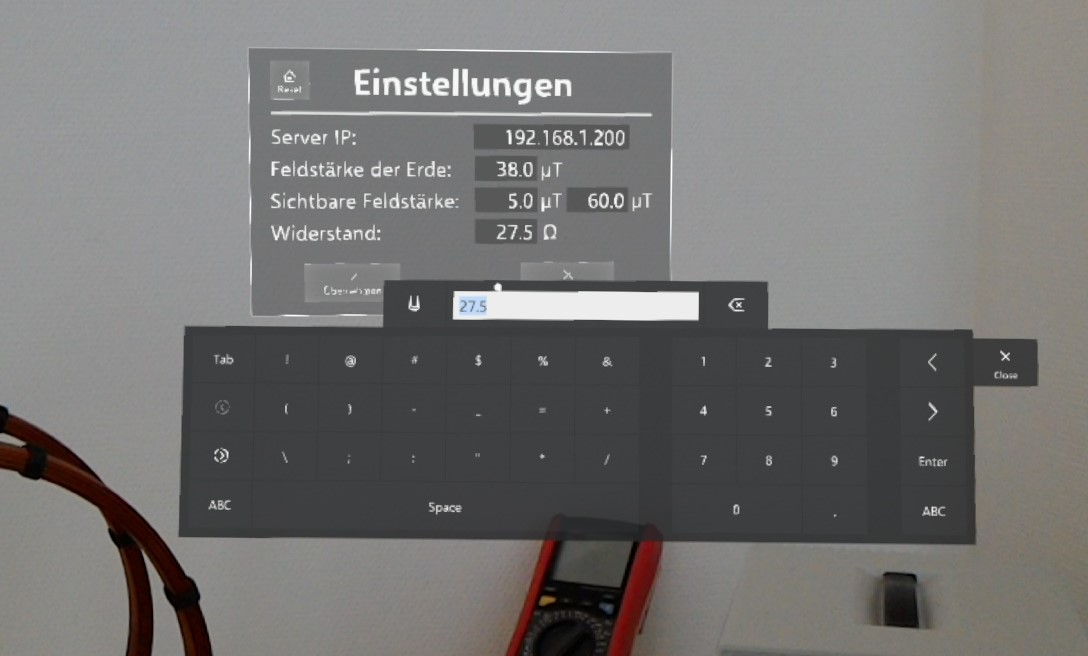
\includegraphics[width=0.8\textwidth]{images/HL/settings_c.jpg}\\
	\scriptsize Einstellungen mit aktiver Tastatur.
	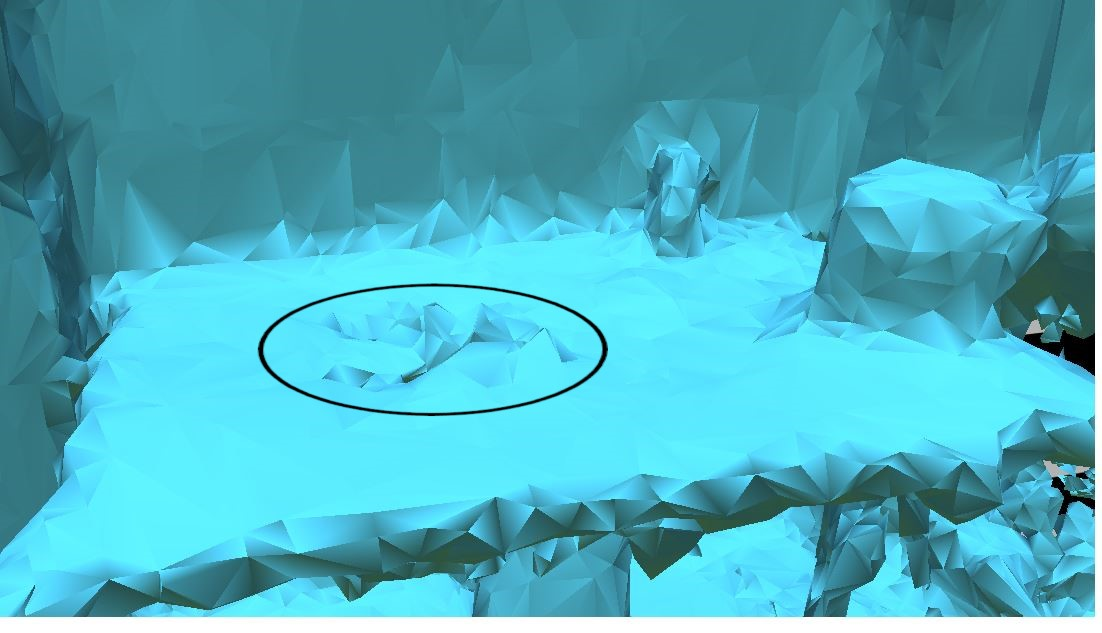
\includegraphics[width=0.8\textwidth]{images/HL/mesh.JPG}\\
	\scriptsize Einstellungen mit aktiver Tastatur.	
\end{minipage}
\end{frame}

\part{Ergebnisse}
\label{part:results}
\begin{frame}[fragile]{Dargestellte Informationen}
\begin{itemize}
	\item Visualisierung der Komponenten des Magnetfeldes in zwei Darstellungen und in Echtzeit
	\item Darstellung einer vorberechneten Lösung für eine ausgewählte Ebene des Feldes der Spule
	\item Kennzeichnung der Stromrichtung
	\item Integration einer virtuellen Kompass-Skala mit Hervorhebung wichtiger Zustände
	\item Einbettung einer virtuellen Kompassnadel auf Basis theoretischer Werte
	\item Numerische Darstellung gemessener und berechneter Echtzeitdaten
\end{itemize}
\end{frame}

\begin{frame}[fragile]{Technische Bewertung}

\setlength\extrarowheight{1pt}
\def\arraystretch{1.1}
\begin{table}
	\centering
	\begin{tabular}{m{5.0cm}|l}
		Kriterium & Bewertung \\
		\hline
		\hline
		Framerate & Optimal\\
		\hline
		Stabilität & Fast optimal\\
		\hline
		Positionierung & Fast optimal\\
		\hline
		Komfortzone & Optimal\\
		\hline
		Tiefen Wechsel & Fast optimal\\
		\hline
		FoV-Grenzen & Optimal\\
		\hline
		Input Interaction Clarity & Erfüllt\\
		\hline
		Anpassung an Nutzerposition & Optimal\\
	\end{tabular}
\end{table}
\scriptsize Bewertung anhand von Qualitätskriterien der Dokumentation. Stufen: ''Optimal'', ''Erfüllt'' und ''Nicht erfüllt''.
\end{frame}

\begin{frame}[fragile]{Performance}
\begin{figure}
	\vspace{-20px}
	\hspace{100px}
	\centering
	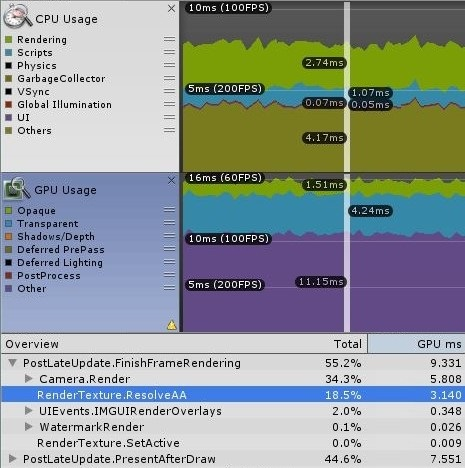
\includegraphics[width=0.6\textwidth]{images/performance/profile_MSAA_on_cut.jpg}\\
	\scriptsize Unity's Profiler zeigt Details zur Renderdauer auf CPU und GPU mit aktivem MSAA.
\end{figure}
\end{frame}

\part{Ausblick}
\label{part:future}
\begin{frame}[fragile]{Erweiterungen}
\usebeamerfont{frametitle}\textcolor{blue}{Inhaltlich:} \usebeamerfont{text}\textit{Weitere Lerninhalte integrieren}
\begin{itemize}
	\item Weitere Inhalte, z.B. Rechte-Hand-Regel
	\item Weitere Experimente, z.B. Ablenkung eines Elektronenstrahles
\end{itemize}
\pause
\vskip 1em
\usebeamerfont{frametitle}\textcolor{blue}{Technisch:} \usebeamerfont{text}\textit{Portierung für HoloLens 2}
\begin{itemize}
	\item Auflösung x4 pro Auge, Sichtfeld x2 (Fläche)
	\item Tragekomfort und Interaktion verbessert
\end{itemize}

\vspace{50px}
\end{frame}



\part{Diskussion}
\begin{frame}[fragile]{}
Vielen Dank für Ihre Aufmerksamkeit!

\vspace{1em}
\hspace{1em} Fragen?
\end{frame}


\end{document}
